\section{Results}\label{sec:results}

\subsection{Clean performance and seed variability}

ResNet-50 achieves higher clean accuracy with less variation across seeds under the executed recipes. Mean final-test accuracy is 98.63\% for ResNet-50 and 96.77\% for ViT-Small/16, with sample SDs of 0.04 and 1.21 percentage points, respectively. Macro-F1 follows the same ordering (Table \ref{tab:clean}). These clean scores provide the reference for measuring transformation effects.

\stopcolumns
\noindent\begin{minipage}[t]{\dimexpr(\textwidth-\columnsep)/2\relax}
\begin{table}[H]
\centering
\caption{Clean final-test performance, mean $\pm$ sample SD across three seeds. Accuracy and macro-F1 are percentages; ECE, Brier and NLL use their native scales. Each run evaluates 4,050 sources. Bold marks the better model for each metric; higher is better for accuracy and macro-F1, while lower is better for ECE, Brier and NLL.}\label{tab:clean}
\begin{tabular}{lrr}
\toprule
Metric & ResNet-50 & ViT-Small/16 \\
\midrule
Acc. (\%) & \textbf{98.63 $\pm$ 0.04} & 96.77 $\pm$ 1.21 \\
Macro-F1 (\%) & \textbf{98.58 $\pm$ 0.03} & 96.66 $\pm$ 1.24 \\
ECE & \textbf{0.0080 $\pm$ 0.0005} & 0.0116 $\pm$ 0.0042 \\
Brier & \textbf{0.0218 $\pm$ 0.0009} & 0.0502 $\pm$ 0.0165 \\
NLL & \textbf{0.0577 $\pm$ 0.0038} & 0.1064 $\pm$ 0.0220 \\
\bottomrule
\end{tabular}

\end{table}

\end{minipage}\hfill\begin{minipage}[t]{\dimexpr(\textwidth-\columnsep)/2\relax}
ResNet's mean expected calibration error (ECE) is 0.0080, versus 0.0116 for ViT, using 15 equal-width confidence bins. Brier score and negative log-likelihood also favor ResNet. Calibration and accuracy nevertheless measure different properties: the lowest-accuracy ViT seed has ECE 0.0067, lower than that of the highest-accuracy ViT seed. A small aggregate calibration gap can coexist with lower accuracy. ECE also depends on binning and the evaluated population \cite{calibration}.

ViT seed 17 attains 98.15\% clean accuracy, while seeds 29 and 43 attain 96.25\% and 95.90\%. All three contribute to the mean. The selected validation epochs and learning curves document this variation across runs, although they do not identify its cause.
\end{minipage}\par\startcolumns

\subsection{RQ1: sensitivity depends strongly on the transformation family}

Resolution reduction produces the largest deterioration on the tested dose grid. ResNet accuracy falls from 87.89\% at mild reduction to 49.47\% at moderate and 12.94\% at severe reduction. ViT falls from 92.89\% to 77.17\% and 43.00\%, respectively. ViT therefore retains higher accuracy at all three tested resolution levels despite its lower clean accuracy. Figure \ref{fig:prediction} shows accuracy alongside JS divergence, separating label correctness from changes in the probability distribution.

\stopcolumns
\noindent\begin{minipage}{\textwidth}
\centering
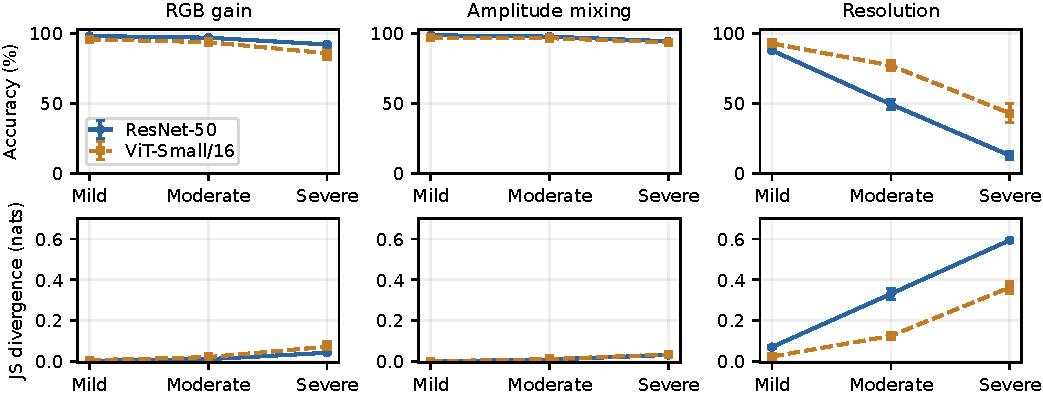
\includegraphics[width=\textwidth]{figures/prediction_response_compact.pdf}
\captionof{figure}{Prediction response across the three frozen doses of each family. Points show means across three seeds, and error bars show sample SD. Each condition uses 4,050 sources per run. Lines connect the evaluated doses; intermediate severities were not measured.}\label{fig:prediction}
\end{minipage}
\par\startcolumns


ResNet retains the advantage under the other two families. Under severe RGB gains, accuracy is 92.14\% for ResNet and 85.85\% for ViT; under severe amplitude mixing, the means are 94.41\% and 93.59\%. Model performance must therefore be described by transformation family. The intervention scales are not perceptually matched, and severe resolution reduction may remove information needed to identify the original class.

Table \ref{tab:contrasts} reports severe-minus-mild effects for matched source images. ResNet's mean resolution JS increase is 0.5219 nats, a large change within the possible JS range of 0 to \(\log 2\). Its RGB-gain and amplitude-mixing increases are much smaller. Label inconsistency, distributional change, and normalized feature change have different units, so their numerical magnitudes should be interpreted within each metric.

\stopcolumns
\noindent\begin{minipage}{\textwidth}
\centering
\captionof{table}{Primary paired severe-minus-mild effects, mean $\pm$ sample SD across seeds. Positive values indicate increasing instability. JS uses natural logarithms; ECDF is on a 0--1 percentile scale. Each per-seed contrast uses the same 4,050 sources. Within each family, bold marks the lower sensitivity value; displayed ties are bold for both models.}\label{tab:contrasts}
\begin{tabular}{llrrr}
\toprule
Model & Family & $\Delta$ inconsistency (pp) & $\Delta$ JS (nats) & $\Delta$ ECDF \\
\midrule
ResNet-50 & RGB gain & \textbf{6.4527 $\pm$ 0.9056} & \textbf{0.0397 $\pm$ 0.0050} & \textbf{0.0028 $\pm$ 0.0008} \\
ResNet-50 & Amplitude mixing & \textbf{5.1276 $\pm$ 0.1918} & \textbf{0.0320 $\pm$ 0.0015} & \textbf{0.0015 $\pm$ 0.0003} \\
ResNet-50 & Resolution & 75.3086 $\pm$ 3.9397 & 0.5219 $\pm$ 0.0146 & 0.6131 $\pm$ 0.0361 \\
ViT-Small/16 & RGB gain & 11.1440 $\pm$ 3.3825 & 0.0660 $\pm$ 0.0220 & 0.0054 $\pm$ 0.0043 \\
ViT-Small/16 & Amplitude mixing & 5.8272 $\pm$ 0.2848 & 0.0335 $\pm$ 0.0008 & \textbf{0.0015 $\pm$ 0.0002} \\
ViT-Small/16 & Resolution & \textbf{51.3498 $\pm$ 6.6212} & \textbf{0.3376 $\pm$ 0.0354} & \textbf{0.0874 $\pm$ 0.0069} \\
\bottomrule
\end{tabular}

\end{minipage}
\par\startcolumns


The lowest dose can also produce a small accuracy increase. Mean mild amplitude-mixing accuracy is 98.73\% for ResNet and 97.13\% for ViT, slightly above their respective clean means. Accuracy can rise when corrections of initially wrong predictions outnumber correct-to-incorrect transitions. Label consistency records both kinds of changes. The observed increases are descriptive outcomes on this held-out partition; they do not establish that amplitude mixing would improve generalization if used during training.

\subsection{RQ2: normalized feature stability and prediction stability are not interchangeable}

Resolution reduction also produces the largest representation changes within each model (Figure \ref{fig:representation}). At severe reduction, ResNet's mean raw cosine similarity is 0.3929 and its ECDF instability is 0.6202; ViT's corresponding values are 0.5550 and 0.0876. The lower ViT ECDF value places its displacement at a lower percentile of its own different-class control distribution. Because the reference distributions are model-specific, the percentiles do not equate absolute distances in the 384- and 2,048-dimensional spaces.

\stopcolumns
\noindent\begin{minipage}{\textwidth}
\centering
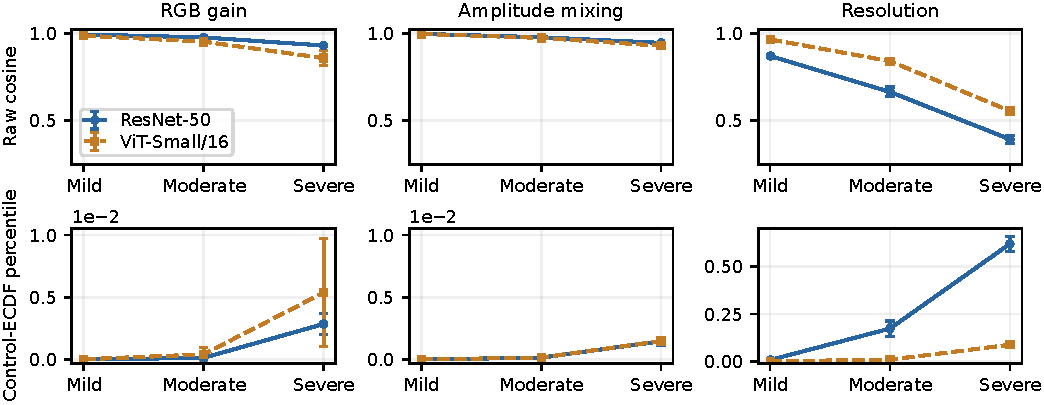
\includegraphics[width=\textwidth]{figures/representation_response_compact.pdf}
\captionof{figure}{Raw within-model cosine (top) and validation-control ECDF instability (bottom), shown as mean and sample SD across seeds. The bottom panels use different scales because RGB gain and amplitude mixing occupy the ECDF lower tail. Near-zero percentiles can coexist with changed predictions. Larger ECDF values indicate greater displacement relative to the run's controls.}\label{fig:representation}
\end{minipage}
\par\startcolumns


Under resolution reduction, the paired increase in normalized instability is 0.6131 $\pm$ 0.0361 for ResNet and 0.0874 $\pm$ 0.0069 for ViT (mean $\pm$ sample SD). Averaging the ViT-minus-ResNet difference-in-differences over all three families gives -0.1744, with a stored two-level bootstrap 95\% CI of [-0.1851, -0.1633]. The group-wise aggregate Wilcoxon result is reported as \(p<0.001\); its Holm family contains only the single active model pair. Resolution dominates this aggregate, so the average does not describe an equal effect across RGB gain, amplitude mixing, and resolution reduction.

Severe RGB gains illustrate why normalized feature stability and prediction stability can diverge. Mean ECDF instability is only 0.00285 for ResNet and 0.00537 for ViT, yet label consistency falls to 92.61\% and 86.77\%. Features can remain close relative to different-class controls while crossing a decision boundary. The raw-cosine panels in Figure \ref{fig:representation} retain within-model changes that are compressed near the ECDF floor.

Figure \ref{fig:scatter} relates confidence drop to normalized representation instability for individual pairs. Each panel contains 109,350 non-sham observations, pooling three seeds and nine conditions for 4,050 sources. In both models, a dense band near the ECDF floor spans a range of confidence changes. A low control percentile therefore does not determine the size of the confidence change. Sources appear repeatedly across seeds and conditions, so the points are dependent observations; the display does not support a causal interpretation.

\stopcolumns
\noindent\begin{minipage}{\textwidth}
\centering
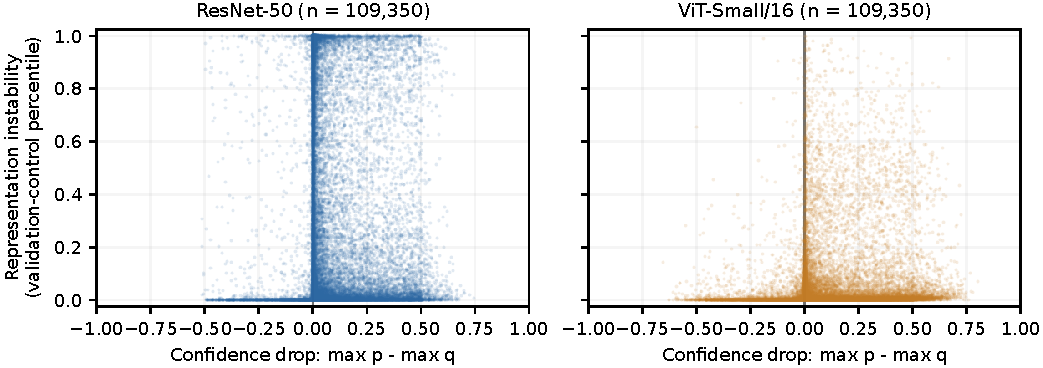
\includegraphics[width=\textwidth]{figures/confidence_representation_scatter_compact.pdf}
\captionof{figure}{Confidence drop and representation instability for all non-sham pairs: 109,350 observations per model (4,050 sources, nine conditions, three seeds). Positive horizontal values indicate a confidence decrease; negative values indicate an increase. The vertical coordinate is a validation-control percentile, not a failure probability. Both panels share scales and include clean errors. Sources recur across seeds and conditions, so observations are dependent. No correlation test is attached to this display.}\label{fig:scatter}
\end{minipage}
\par\startcolumns


The scatter includes initially incorrect predictions. RQ3 restricts evaluation to initially correct sources and tests whether the representation feature improves detection of their subsequent failures.

\subsection{RQ3: representation adds discrimination beyond the specified output baseline}

Adding normalized representation instability improves both AP and AUROC in every model/seed comparison. Mean paired AP gains are 0.432 $\pm$ 0.113 for ResNet and 0.402 $\pm$ 0.032 for ViT. Mean paired AUROC gains are 0.166 $\pm$ 0.087 and 0.114 $\pm$ 0.023. The $\pm$ values are sample SDs across three seeds. Table \ref{tab:detectors} gives all five score variants and the paired gains.

\stopcolumns
\noindent\begin{minipage}{\textwidth}
\centering
\captionof{table}{Failure-discrimination scores and paired gains, mean $\pm$ sample SD across three seeds. AP denotes average precision. Populations and prevalence differ by model/seed (Appendix~\ref{app:detector}); paired gains compare detectors on the same rows within each run. Within each model, bold marks the highest AP or AUROC among the five absolute score variants.}\label{tab:detectors}
\begin{tabular}{lrrrr}
\toprule
& \multicolumn{2}{c}{ResNet-50} & \multicolumn{2}{c}{ViT-Small/16} \\
Score / paired gain & AP & AUROC & AP & AUROC \\
\midrule
Confidence & 0.513 $\pm$ 0.102 & 0.819 $\pm$ 0.084 & 0.489 $\pm$ 0.028 & 0.867 $\pm$ 0.027 \\
Entropy & 0.513 $\pm$ 0.105 & 0.818 $\pm$ 0.085 & 0.498 $\pm$ 0.029 & 0.869 $\pm$ 0.026 \\
Output only & 0.507 $\pm$ 0.107 & 0.818 $\pm$ 0.085 & 0.496 $\pm$ 0.028 & 0.869 $\pm$ 0.026 \\
Output + representation & \textbf{0.939 $\pm$ 0.006} & \textbf{0.983 $\pm$ 0.001} & \textbf{0.898 $\pm$ 0.020} & \textbf{0.983 $\pm$ 0.007} \\
Representation only & 0.918 $\pm$ 0.008 & 0.966 $\pm$ 0.005 & 0.878 $\pm$ 0.032 & 0.955 $\pm$ 0.017 \\
$\Delta$ AP & 0.432 $\pm$ 0.113 & -- & 0.402 $\pm$ 0.032 & -- \\
$\Delta$ AUROC & -- & 0.166 $\pm$ 0.087 & -- & 0.114 $\pm$ 0.023 \\
\bottomrule
\end{tabular}

\end{minipage}
\par\startcolumns


Figure \ref{fig:detectors} shows the within-seed source-group bootstrap intervals for the paired gains. Every displayed interval lies above zero, although the twelve intervals do not provide simultaneous coverage.

\stopcolumns
\noindent\begin{minipage}{\textwidth}
\centering
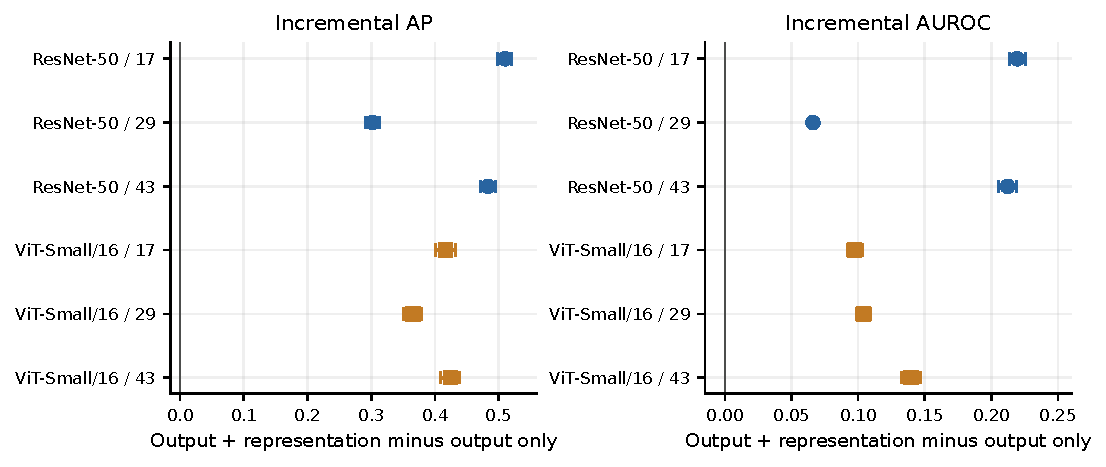
\includegraphics[width=\textwidth]{figures/detector_deltas.pdf}
\captionof{figure}{Incremental detector performance by training seed. Points show paired gains from adding representation to the two output features. Bars are stored 95\% source-group bootstrap CIs from 2,000 replicates, conditional on each trained model and fitted detector. Every interval excludes zero; coverage is individual rather than simultaneous.}\label{fig:detectors}
\end{minipage}
\par\startcolumns


The eligible population comprises 35,937--35,964 pairs per ResNet seed and 34,956--35,775 per ViT seed. Positive prevalence is 18.05--18.55\% for ResNet and 10.30--13.12\% for ViT. Both population size and prevalence depend on which sources each run classifies correctly before transformation and which then fail. Since AP depends on prevalence, the absolute scores do not provide a population-matched ranking of the models. Comparing the two detectors within each run holds the population fixed. Appendix \ref{app:detector} reports the exact counts and prevalence.

The representation-only score achieves mean AP of approximately 0.918 for ResNet and 0.878 for ViT. Adding the two output features raises the respective means to approximately 0.939 and 0.898. Much of the gain over the output-only baseline is therefore present in the representation score alone. The evidence supports this feature's value within the tested logistic model, without establishing a need for a more complex fusion architecture. Richer output-only baselines remain an open comparison.

The ResNet output baseline varies substantially across seeds: its AUROC is 0.765, 0.916, and 0.772 for seeds 17, 29, and 43. The augmented detector remains at approximately 0.982--0.985 across the same runs. The resulting gain is consequently smaller for seed 29, as reflected in the per-seed intervals and the SD of the paired gains.

The pooled detector task gives each source one pair in each of the nine conditions. Differences in condition difficulty, especially the high failure rate under resolution reduction, can contribute to pooled discrimination. Equal performance within every family, class, or severity cannot be inferred from that score. The saved condition-prevalence tables document the mixture, but the pooled summary does not supply condition-specific AUROC estimates. Detector calibration, operating thresholds, and performance under deployment shifts were also not established by this evaluation.

\subsection{Controls and class-wise behavior}

Sham conditions retain label consistency of one across all six runs, confirming that the identity processing paths preserve predicted labels. The check does not extend to semantic preservation under nonzero perturbations. Different-class controls supply the ECDF reference scale using known labels and content exclusions; their purpose is normalization rather than an independent adversarial stress test.

Figure \ref{fig:classes} breaks down severe-condition label consistency by the ten original classes. Each cell averages the same three seeds and includes all final-test sources in the class, including clean errors. The denominator therefore differs from RQ3. The resolution columns show substantial variation across classes that is concealed by a single model mean. All classes are shown, and the cell differences are descriptive; no class-wise significance tests were performed.

\stopcolumns
\noindent\begin{minipage}{\textwidth}
\centering
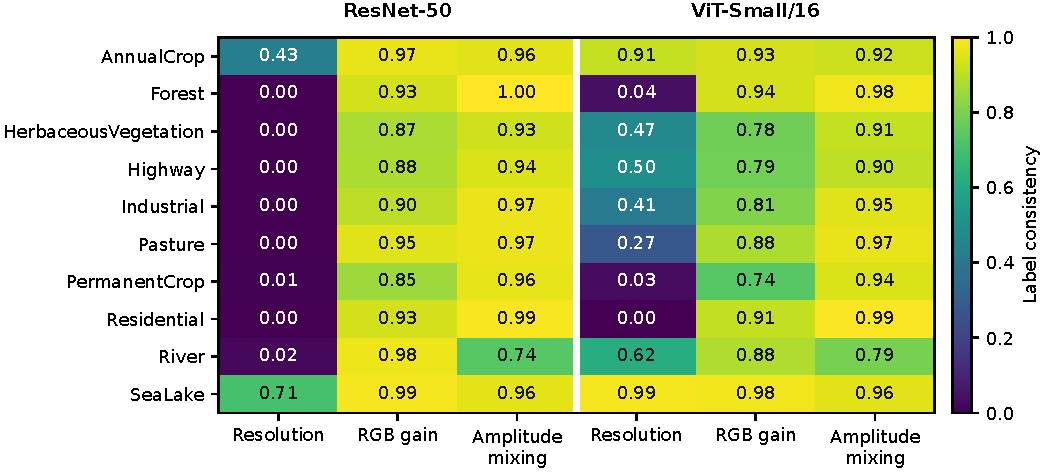
\includegraphics[width=\textwidth]{figures/class_heatmap_compact.pdf}
\captionof{figure}{Severe-condition label consistency by class, averaged across three seeds. Each cell includes all class sources, including clean errors. Consistency measures agreement with the clean prediction; accuracy would compare with the dataset label. The shared scale runs from zero (purple) to one (yellow), with rounded values printed in each cell. Class sample counts appear in Appendix~\ref{app:counts}. Cell differences are descriptive and have no class-wise significance tests.}\label{fig:classes}
\end{minipage}
\par\startcolumns


Appendix \ref{app:qualitative} illustrates four failures selected for high clean confidence and mild transformation severity. All four involve RGB gains and prediction switches between PermanentCrop and HerbaceousVegetation. Clean confidence exceeds 0.99 in each case, yet the transformed prediction is incorrect relative to the dataset label. The selection illustrates the failure definition without estimating its frequency. Appendix \ref{app:attention} presents the related attention rollout and documents its rendering repair.
